%%%%%%%%%%%%%%%%%%%%%%%%%%%%%%%%%%%%%%%%%
% Classicthesis Typographic Thesis
% LaTeX Template
% Version 1.3 (15/2/14)
%
% This template has been downloaded from:
% http://www.LaTeXTemplates.com
%
% Original author:
% André Miede (http://www.miede.de)
%
% License:
% CC BY-NC-SA 3.0 (http://creativecommons.org/licenses/by-nc-sa/3.0/)
%
% General Tips:
% 1) Make sure to edit the classicthesis-config.file
% 2) New enumeration (A., B., C., etc in small caps): \begin{aenumerate}
% \end{aenumerate}
% 3) For margin notes: \marginpar or \graffito{}
% 4) Do not use bold fonts in this style, it is designed around them
% 5) Use tables as in the examples
% 6) See classicthesis-preamble.sty for useful commands
%
%%%%%%%%%%%%%%%%%%%%%%%%%%%%%%%%%%%%%%%%%

%-------------------------------------------------------------------------------
%	PACKAGES AND OTHER DOCUMENT CONFIGURATIONS
%-------------------------------------------------------------------------------

\documentclass[
		twoside,openright,titlepage,numbers=noenddot,headinclude,1headlines,
                footinclude=true,cleardoublepage=empty,
                BCOR=5mm,paper=a4,fontsize=11pt, % Binding correction, paper type
                american, % Languages
                ]{scrreprt}

% Includes the file which contains all the document configurations and packages
% - make sure to edit this file

\input{tex/classicthesis-config}
% use upquote if available, for straight quotes in verbatim environments
\IfFileExists{upquote.sty}{\usepackage{upquote}}{}
% use microtype if available
\IfFileExists{microtype.sty}{\usepackage{microtype}}{}
\usepackage{biblatex}
\usepackage{color}
\usepackage{fancyvrb}
\newcommand{\VerbBar}{|}
\newcommand{\VERB}{\Verb[commandchars=\\\{\}]}
\DefineVerbatimEnvironment{Highlighting}{Verbatim}{commandchars=\\\{\},fontsize=\small}
% Add ',fontsize=\small' for more characters per line
\usepackage{framed}
\definecolor{shadecolor}{RGB}{248,248,248}
\newenvironment{Shaded}{\begin{snugshade}}{\end{snugshade}}
\newcommand{\KeywordTok}[1]{\textcolor[rgb]{0.13,0.29,0.53}{\textbf{{#1}}}}
\newcommand{\DataTypeTok}[1]{\textcolor[rgb]{0.13,0.29,0.53}{{#1}}}
\newcommand{\DecValTok}[1]{\textcolor[rgb]{0.00,0.00,0.81}{{#1}}}
\newcommand{\BaseNTok}[1]{\textcolor[rgb]{0.00,0.00,0.81}{{#1}}}
\newcommand{\FloatTok}[1]{\textcolor[rgb]{0.00,0.00,0.81}{{#1}}}
\newcommand{\CharTok}[1]{\textcolor[rgb]{0.31,0.60,0.02}{{#1}}}
\newcommand{\StringTok}[1]{\textcolor[rgb]{0.31,0.60,0.02}{{#1}}}
\newcommand{\CommentTok}[1]{\textcolor[rgb]{0.56,0.35,0.01}{\textit{{#1}}}}
\newcommand{\OtherTok}[1]{\textcolor[rgb]{0.56,0.35,0.01}{{#1}}}
\newcommand{\AlertTok}[1]{\textcolor[rgb]{0.94,0.16,0.16}{{#1}}}
\newcommand{\FunctionTok}[1]{\textcolor[rgb]{0.00,0.00,0.00}{{#1}}}
\newcommand{\RegionMarkerTok}[1]{{#1}}
\newcommand{\ErrorTok}[1]{\textbf{{#1}}}
\newcommand{\NormalTok}[1]{{#1}}

% prevent graphics from overflowing
\usepackage{graphicx}
\makeatletter
\def\maxwidth{\ifdim\Gin@nat@width>\linewidth\linewidth\else\Gin@nat@width\fi}
\def\maxheight{\ifdim\Gin@nat@height>\textheight\textheight\else\Gin@nat@height\fi}
\makeatother
\setkeys{Gin}{width=\maxwidth,height=\maxheight,keepaspectratio}

%%%%%%%%%% Version 1.0 %%%%%%%%%%

% Model:
% \newcommand{\nDomains}{D}
% \newcommand{\indexDomain}{i}
% \newcommand{\directStat}{y}
% \newcommand{\directStatIndexed}{y_{\indexDomain}}
% \newcommand{\trueStat}{\mu}
% \newcommand{\trueStatIndexed}{\mu_{\indexDomain}}
% \newcommand{\indexUnit}{j}
% \newcommand{\nUnitIndexed}{n_\indexDomain}

% Sampling-Error
% \newcommand{\samplingError}{e}
% \newcommand{\samplingErrorIndexed}{e_{\indexDomain}}
% \newcommand{\samplingErrorUnitIndexed}{e_{\indexDomain\indexUnit}}
% \newcommand{\samplingVariance}{\sigma_e^2}
% \newcommand{\samplingVarianceIndexed}{\sigma_{e, i}^2}
% \newcommand{\samplingSD}{\sigma_e}
%
% % Uni Error
% \newcommand{\unitError}{e}
%
% % Random Effects
% \newcommand{\randomEffectIndexed}{v_{\indexDomain}}
% \newcommand{\randomEffect}{v}
% \newcommand{\randomEffectVariance}{\sigma_v^2}
% \newcommand{\randomEffectSD}{\sigma_v}
% \newcommand{\RandomEffect}{\mathbf{v}}

% Regressors
% \newcommand{\xArea}{x_{\indexDomain}}
% \newcommand{\xUnit}{x_{\indexDomain\indexUnit}}
% \newcommand{\X}{\mathbf{X}}
% \newcommand{\indexRegressor}{p}
% \newcommand{\nRegressor}{P}

% Math Operators
% \DeclareMathOperator{\tr}{tr}
% \DeclareMathOperator{\diag}{diag}

% Matrix Notation
% \newcommand{\IdentityMatrix}{\mathbf{I}}


% Fixed Point
\newcommand{\aFH}{\psi(\mathbf{r})^\top \mathbf{U}^{\frac{1}{2}}\mathbf{V}^{-1}\frac{\partial\mathbf{V}}{\partial\theta}\mathbf{V}^{-1}\mathbf{U}^{\frac{1}{2}} \psi(\mathbf{r})}


%%%%%%%%%% Version 2.0 %%%%%%%%%%
% constants:

\newcommand{\sige}{\sigma_{ei}^2}
\newcommand{\sigre}{\sigma_{u}^2}
\newcommand{\re}{u}
\newcommand{\half}{\frac{1}{2}}

% funs:
\DeclareMathOperator{\tr}{tr}
\newcommand{\Tr}[1]{tr\left(#1\right)}
\DeclareMathOperator{\diag}{diag}
\newcommand{\Diag}[1]{diag\left(#1\right)}
\newcommand{\Paran}[1]{\left(#1\right)}

% formats:
\newcommand{\Distr}[1]{\mathcal{#1}}
\newcommand{\mat}[1]{\mathbf{#1}}
\newcommand{\pmat}[1]{\boldsymbol{#1}}
\newcommand{\Exp}[1]{\mathbb{#1}}

% subscripts:
\newcommand{\si}[1]{#1_i}
\newcommand{\sij}[1]{#1_{ij}}

% references
\newcommand{\eq}[1]{(\ref{#1})}

\newcommand{\textrrmse}{Boxplot with Relative Root Mean Squared Error (RRMSE)}
\newcommand{\textrbias}{Boxplot with Relative Bias (RBIAS)}


\begin{document}

\frenchspacing % Reduces space after periods to make text more compact

\raggedbottom % Makes all pages the height of the text on that page

\selectlanguage{american} % Select your default language - e.g. american or ngerman

%\renewcommand*{\bibname}{new name} % Uncomment to change the name of the bibliography
%\setbibpreamble{} % Uncomment to include a preamble to the bibliography - some text before the reference list starts

\pagenumbering{roman} % Roman page numbering prior to the start of the thesis content (i, ii, iii, etc)

\pagestyle{plain} % Suppress headers for the pre-content pages

%-------------------------------------------------------------------------------
%	PRE-CONTENT THESIS PAGES
%-------------------------------------------------------------------------------

% Title Page

\begin{titlepage}

\begin{addmargin}[-1cm]{-3cm}
\begin{center}
\large

\hfill
\vfill

\begingroup
\color{Maroon}
\spacedallcaps{\myTitlei} \\  % Thesis title
\spacedallcaps{\myTitleii} \\
\medskip
\endgroup

\spacedlowsmallcaps{\mySubtitle}

\bigskip

\spacedlowsmallcaps{\myName} % Your name

\vfill

%\includegraphics[width=6cm]{figs/FULogo_RGB} \\ \medskip % Picture

% \\ \medskip % Thesis subtitle
\myDegree \\
% \myDepartment \\
\myFaculty \\
\myUni \\ \bigskip

\myTime\ -- \myVersion % Time and version

\vfill

\end{center}
\end{addmargin}

\end{titlepage}
 % Main title page

\include{tex/Titleback} % Back of the title page

% \cleardoublepage\include{tex/Dedication} % Dedication page

% \cleardoublepage\include{FrontBackMatter/Foreword} % Uncomment and create a Foreword.tex to include a foreword

% \cleardoublepage% Abstract

\pdfbookmark[1]{Abstract}{Abstract} % Bookmark name visible in a PDF viewer

\begingroup
\let\clearpage\relax
\let\cleardoublepage\relax
\let\cleardoublepage\relax

\chapter{Abstract} % Abstract name

Short summary of the contents\dots

\endgroup

\vfill
\pagebreak

% Zusammenfassung

\pdfbookmark[1]{Zusammenfassung}{Zusammenfassung} % Bookmark name visible in a PDF viewer

\begingroup
\let\clearpage\relax
\let\cleardoublepage\relax
\let\cleardoublepage\relax

\chapter{Zusammenfassung} % Abstract name
\selectlanguage{ngerman}

Kurze Zusammenfassung\dots

\endgroup

\vfill

\selectlanguage{british}
 % Abstract page

% \cleardoublepage% Publications - a page listing research articles written using content in the thesis

\pdfbookmark[1]{Publications}{Publications} % Bookmark name visible in a PDF viewer

\chapter*{Publications} % Publications page text

Some ideas and figures have appeared previously in the following publication:

\bigskip

\noindent Warnholz, S. and T. Schmid (2016). “Simulation Tools for Small Area
Estimation: Introducing the R-package saeSim”. In: \textit{Austrian Journal
of Statistics} 45.1, pp. 55–69.

\bigskip

\noindent The results of this Article are the subject matter of Chapter
\ref{chap:saeSim}. There I state, again, explicitly that these results have been
previously published and how I intend to use them in the context of this Thesis.
 % Publications from the thesis page

% \cleardoublepage\include{tex/Acknowledgments} % Acknowledgements page

\pagestyle{scrheadings} % Show chapter titles as headings

\cleardoublepage\include{tex/Contents} % Contents, list of figures/tables/listings and acronyms

\cleardoublepage

\pagenumbering{arabic} % Arabic page numbering for thesis content (1, 2, 3, etc)
%\setcounter{page}{90} % Uncomment to manually start the page counter at an
%arbitrary value (for example if you wish to count the pre-content pages in the
%page count)

\cleardoublepage % Avoids problems with pdfbookmark

%----------------------------------------------------------------------------------------
%	THESIS CONTENT - CHAPTERS
%----------------------------------------------------------------------------------------

%\ctparttext{You can put some informational part preamble text here.} % Text on
%the Part 1 page describing  the content in Part 1

%\part{Some Kind of Manual} % First part of the thesis

%\include{tex/Chapter01} % Chapter 1

%\cleardoublepage % Empty page before the start of the next part

%------------------------------------------------

% \section{new section}\label{new-section}

\begin{itemize}
\itemsep1pt\parskip0pt\parsep0pt
\item
  item

  \begin{itemize}
  \itemsep1pt\parskip0pt\parsep0pt
  \item
    item 1.1
  \item
    item 1.2
  \item
    new item
  \end{itemize}
\end{itemize}

\[
\begin{aligned}
x_i &= y_i \\
x_i + y_i &= y_i
\end{aligned}
\]

cite me: \textcite{Abb97}

\begin{Shaded}
\begin{Highlighting}[]
\NormalTok{x <-}\StringTok{ }\DecValTok{1}
\end{Highlighting}
\end{Shaded}

\begin{Shaded}
\begin{Highlighting}[]
\KeywordTok{plot}\NormalTok{(}\DecValTok{1}\NormalTok{:}\DecValTok{10}\NormalTok{)}
\end{Highlighting}
\end{Shaded}

\begin{figure}[htbp]
\centering
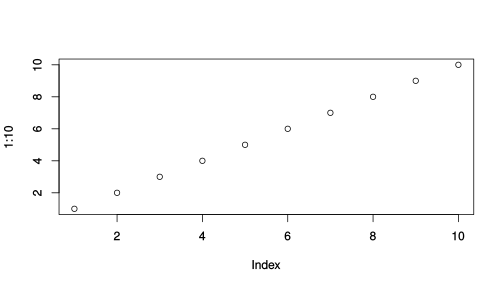
\includegraphics{figs/test/unnamed-chunk-2-1.png}
\caption{plot of chunk unnamed-chunk-2}
\end{figure}


\chapter{Introduction}
\input{Rmd/introduction}

\ctparttext{This is the chapter where I want to present the theoretical concepts
underpinning the development of software and application.}

\part{Theory}\label{part:theory}

\chapter{Small Area Estimation}

\input{Rmd/theory_sae_intro}
\input{Rmd/theory_sae_direct_estimators}
\input{Rmd/theory_sae_blup}
\input{Rmd/theory_sae_area_level}
\input{Rmd/theory_sae_unit_level}
\input{Rmd/theory_sae_robust}

%------------------------------------------------

\chapter{Robust Area Level Models}\label{chap:rfh}

\input{Rmd/theory_rfh_framework}
\input{Rmd/theory_rfh_model}
\input{Rmd/theory_rfh_bias_correction}
\input{Rmd/theory_rfh_mse}
\section{Diagnostic Plots for Robust Predictions}

%------------------------------------------------

\part{Implementation}\label{part:implementation}

\chapter{Implementation}\label{part:implementation}
\input{Rmd/implementation_intro}
\section{Software}
\section{Verification of Results}
\section{Accuracy of Results}
\section{Validation of Results}
\input{Rmd/implementation_validation}

%------------------------------------------------

\ctparttext{This is the part where I will present all results.}
\part{Results}\label{part:results}

\chapter{Numerical Properties}
\section{Accuracy}
\section{Stability}
\section{Speed of Convergence}

\chapter{Simulation Studies}
\section{Model Based Simulation Studies}
\input{Rmd/results_area_level_mc}
\input{Rmd/results_area_level_mse}
\subsection{From Unit to Area Level Data}
\input{Rmd/results_unit_to_area_level_mc}

\section{Design Based Simulation Studies}


%-------------------------------------------------------------------------------
%	THESIS CONTENT - APPENDICES
%-------------------------------------------------------------------------------

\appendix

\part{Appendix} % New part of the thesis for the appendix

%\include{Chapters/Chapter0A} % Appendix A
%\include{Chapters/Chapter0B} % Appendix B - empty template

%-------------------------------------------------------------------------------
%	POST-CONTENT THESIS PAGES
%-------------------------------------------------------------------------------

\cleardoublepage\include{tex/Bibliography} % Bibliography

%\cleardoublepage\include{tex/Colophon} % Colophon

%\cleardoublepage% Declaration

\refstepcounter{dummy}
\pdfbookmark[0]{Declaration}{declaration} % Bookmark name visible in a PDF viewer

\chapter*{Declaration} % Declaration section text

\thispagestyle{empty}

I certify that this work contains no material which has been accepted for the
award of any other degree or diploma in my name, in any university or other
tertiary institution and, to the best of my knowledge and belief, contains no
material previously published or written by another person, except where due
reference has been made in the text.

\bigskip

\noindent\textit{\myLocation, \myTime}

\smallskip

\begin{flushright}
\begin{tabular}{m{5cm}}
\\ \hline
\centering\myName, \today \\
\end{tabular}
\end{flushright}
 % Declaration

%-------------------------------------------------------------------------------

\end{document}
